\chapter{Hot Gas Layer Temperature and Depth}

CFAST simulated all of the chosen experiments.  Details of the comparisons with experimental data, are provided in Appendix A.  The results are organized by quantity as follows:

\begin{itemize}
\item hot gas layer (HGL) temperature and height
\item ceiling jet temperature
\item plume temperature 
\item flame height
\item oxygen and carbon dioxide concentration
\item smoke concentration
\item compartment pressure
\item radiation heat flux, total heat flux, and target temperature
\item wall heat flux and surface temperature
\end{itemize}

Comparisons of the model predictions with experimental measurements are presented as relative differences.  The relative differences are calculated as follows:

\begin{equation}
   \varepsilon = \frac{{\Delta M - \Delta E}}{{\Delta E}} = \frac{{(M_P - M_0)-(E_P - E_0)}}{{(E_P - E_0)}}  \label{eqdixxfeqform} 
\end{equation}

where $\Delta M$ is the difference between the peak value ($M_P$) of the evaluated parameter and its original value ($M_0$), and $\Delta E$ is the difference between the experimental observation ($E_P$) and its original value ($E_0$).  

The measure of model �accuracy� used throughout this study is related to experimental uncertainty. Reference \cite{NRCNUREG1824Experimental}  discusses this issue in detail. In brief, the accuracy of a measurement, for example, a gas temperature, is related to the measurement device, a thermocouple. In addition, the accuracy of the model prediction of the gas temperature is related to the simplified physical description of the fire and the accuracy of the input parameters, especially the specified heat release rate. Ideally, the purpose of a validation study is to determine the accuracy of the model in the absence of any errors related to the measurement of both its inputs and outputs. Because it is impossible to eliminate experimental uncertainty, at the very least a combination of the uncertainty in the measurement of model inputs and output can be used as a yardstick. Dotted lines in figure \ref{fig:HGL_Scatter}  show this combined uncertainty estimate for HGL temperature and layer depth. Corresponding estimates are included for other quantities in later sections. If the numerical prediction falls within the range of uncertainty attributable to both the measurement of the input parameters and the output quantities, it is not possible to further quantify its accuracy. At this stage, it is said that the prediction is within experimental uncertainty.

Note that the calculation of relative difference is based on the temperature rise above ambient, and the layer depth, that is, the distance from the ceiling to where the hot gas layer descends.  Where the model over-predicts the HGL temperature or the depth of the HGL, the relative difference is a positive number. This convention is used throughout this report where the model over-predicts the severity of the fire, the relative difference is positive; where it under-predicts, the difference is negative.

Arguably the most frequent question asked about a fire is, �How hot did it become?�  Temperature in the upper layer of a compartment is an obvious indicator to answer this question.  Peak temperature, time to peak temperature, or time to reach a chosen temperature tenability limit are typical values of interest.  Quality of the prediction (or measurement) of layer interface position is more difficult to quantify.  Although observed in a range of experiments, the two-layer assumption is in many ways just a convenience for modeling.  In experimental measurements, temperature is typically measured with an array of thermocouples from floor to ceiling.  This floor to ceiling temperature profile can then used to estimate a hot gas layer height and the temperature of the upper and lower gas layers \cite{Janssens:1992} \cite{McGrattan:2003} consistent with the two-zone assumption. Appendix A provides details of the calculation.

From a standpoint of hazard, time of descent to a chosen level may be a reasonable criterion (assuming some in the room will then either be forced to crawl beneath the interface to breathe the �clean� atmosphere near the floor or be forced to breath the upper layer gases).  Minimum values may also be used to indicate general agreement.  For the single-room tests with furniture or wall-burning, these are appropriate indicators to judge the comparisons between model and experiment.  For the more-closely steady-state three- and four-room tests with corridor or the multiple-story building tests, a steady-state average may better characterizes the nature of the experiment.

A good prediction of the HGL height is largely a consequence of a good prediction of its temperature because smoke and heat are largely transported together and most numerical models describe the transport of both with the same type of algorithm.  Typically, CFAST slightly over-predicts the HGL temperature, most often within experimental uncertainty.  Hot gas layer height is typically within experimental uncertainty for well-ventilated tests and near floor level for under-ventilated tests where compartments are closed to the outside.  For HGL height, only values from open-door tests are included.  For closed-door tests, visual observations typically show that the HGL fills the entire compartment volume from floor to ceiling, inconsistent with the calculated results for the experimental data.  Thus, the calculated experimental values of HGL height for closed-door tests are not seen as appropriate for comparison to model results.

\section{Model / Experiment Comparisons}

Figure \ref{fig:HGL_Scatter} shows a comparison of predicted and measured values for HGL temperature and depth. Appendix A provides individual graphs of model and experimental values and tables of peak values and relative differences.  

\begin{figure}
\begin{tabular*}{\textwidth}{l@{\extracolsep{\fill}}r}
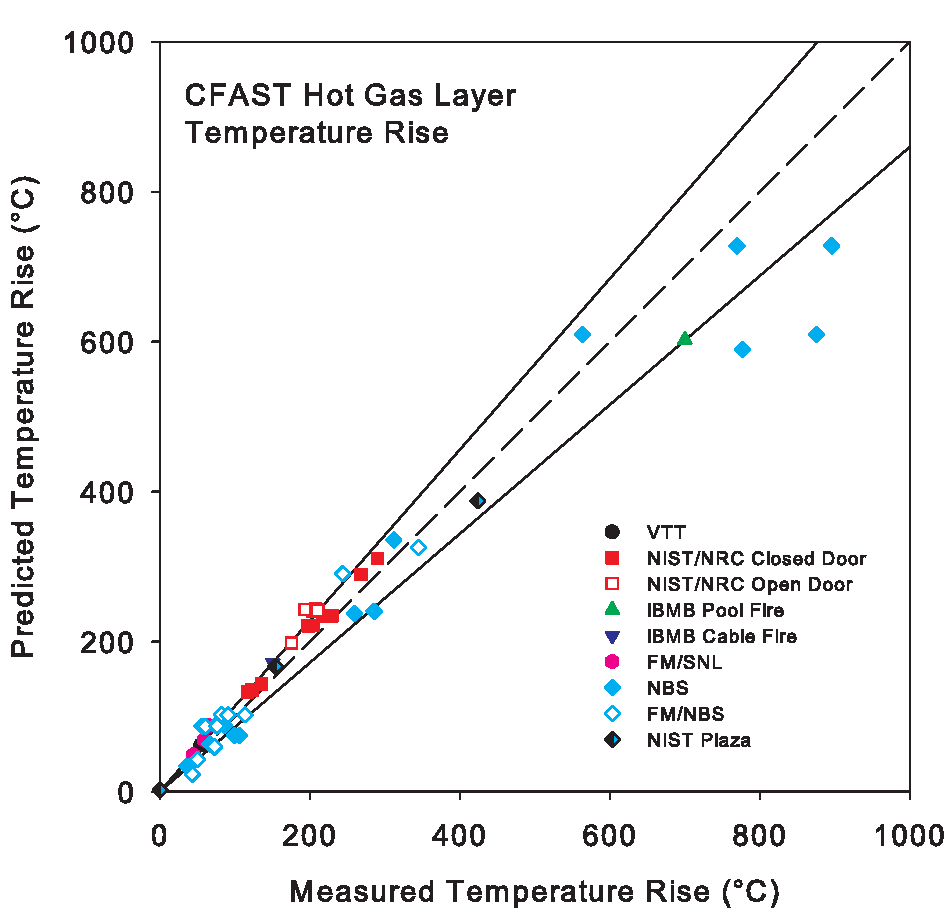
\includegraphics[width=3.0in]{FIGURES/ScatterPlots/HGL_Temp} &
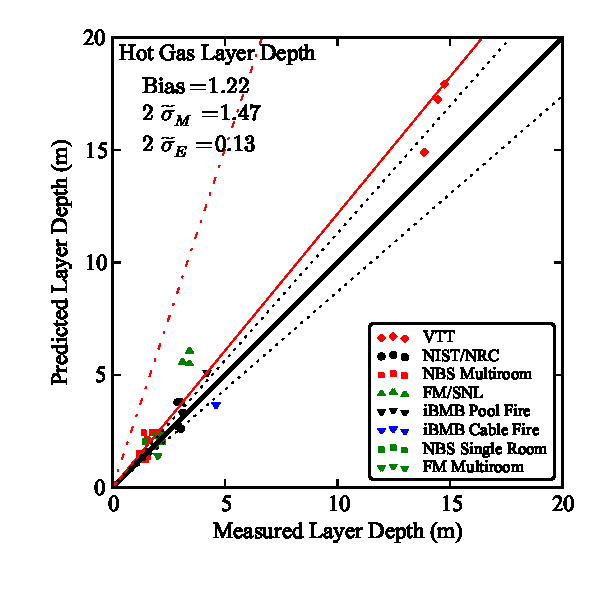
\includegraphics[width=3.0in]{FIGURES/ScatterPlots/HGL_Depth} \\
\multicolumn{2}{c}{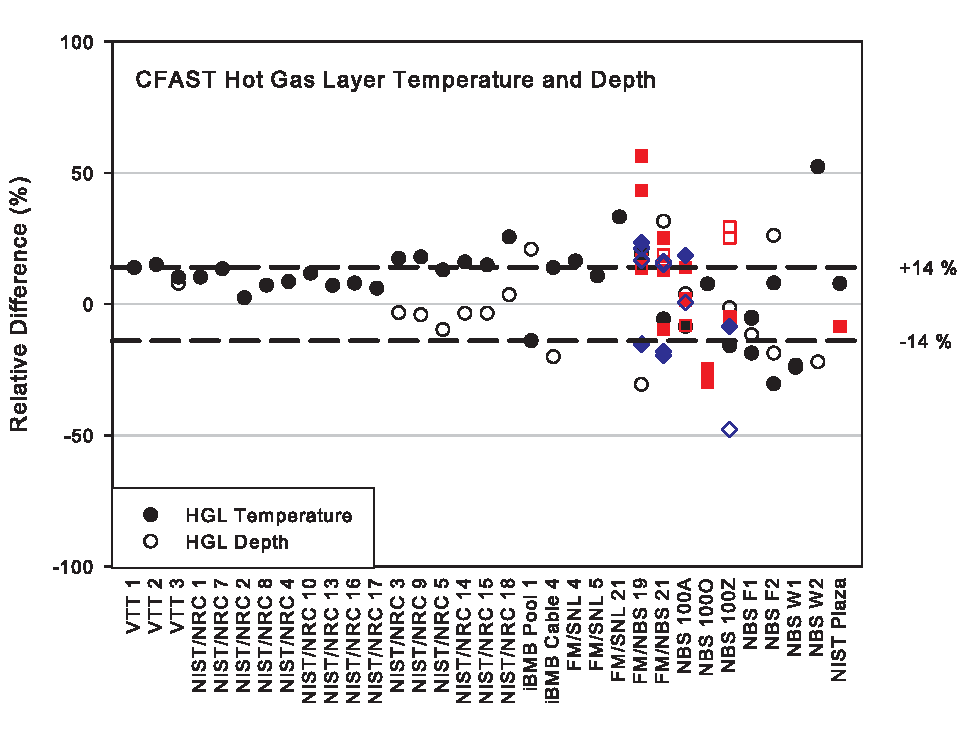
\includegraphics[width=4.5in]{FIGURES/Relative_Diff/HGL}}
\end{tabular*}
\caption{Comparison of Measured and Predicted HGL Temperature and Height.} \label{fig:HGL_Scatter}
\end{figure}

Following is a summary of the accuracy assessment for the HGL predictions of the test series:

\subsubsection{NBS Single Room Tests with Furniture}

For two of the four tests (Tests F1 and F6, tests with a single furniture item in the compartment), the HGL temperature and depth for these tests were calculated separately for two different thermocouple arrays, one located in the front of the compartment and one in the rear. For the other two tests (tests W1 and W2, tests with furniture and a wood wall surface), a single thermocouple array was available.

For the single-room tests, predicted temperatures and layer interface position show obvious
similarities to the measured values. Peak values occurred at similar times with comparable rise
and fall for most comparisons. Interface height for the single-room with wall-burning is a
notable exception. Unlike the model prediction, the experimental measurement did not show the
rise and fall in concert with the temperature measurement. Peak values were typically higher for
upper layer temperature and lower for lower layer temperature and layer interface position.

For the furniture tests, the agreement ranges from a relative difference of -30 \% to 8 \%.  The agreement is quite different for the two arrays in each test. Table \ref{tab:NBS_HGL} shows the relative differences for tests F1 and F6.  For both the layer temperature and layer depth, the difference between the model and experiment changes depending on the measurement location. In the same tests (F1) the values are well within experimental uncertainty at one location and outside for the other.   For test F6, this varies from -30~\% to 8~\% for the temperature and from -19~\% to 26~\% for the layer depth.   For these tests with a post-flashover fire in a small compartment, clearly the assumption of a uniform  upper layer is questionable. Curve shape for the experimental data and model predictions is quite similar.

\begin{table}[h!]
\begin{center}
\caption{Relative Difference for HGL Temperature and Depth for Two Measurement Locations in Two Single-Room Tests}
\label{tab:NBS_HGL}
\vspace{0.1in}
\begin{tabular}{|l|c|c|c|c|}
\hline
Test & Location & Temperature & Layer Depth\\
 & & \% & \% \\ \hline
\hline
\multirow{2}{*}{F1} & A &  -5 & -5 \\
 & B & -19 & -12 \\ 
 \hline
\multirow{2}{*}{F6} & A &   8 & -19 \\
 & B & -30 &  26 \\ 
  \hline
\end{tabular}  
\end{center}
\end{table}

\subsubsection{VTT Large Hall Test Series}

The HGL temperature and depth were calculated from the averaged gas temperatures from three vertical thermocouple arrays.  Ten thermocouples in each vertical array, spaced 2 m apart in the lower two-thirds of the hall, and 1 m apart near the ceiling were used to determine layer temperatures and depth.  

CFAST predicts the HGL temperature and height near experimental uncertainty for all three tests, with relative differences ranging from 10 \% to 15 \%, depending on the test. Relative differences are shown in figure \ref{fig:HGL_Scatter}.

\subsubsection{NIST/NRC Test Series}

The NIST/NRC series consisted of 15 liquid spray fire tests with different heat release rates, pan locations, and ventilation conditions.  Gas temperatures were measured using seven floor-to-ceiling thermocouple arrays (or ``trees'') distributed throughout the compartment.  The average hot gas layer temperature and height were calculated using thermocouple Trees 1, 2, 3, 5, 6 and 7. Tree 4 was not used because one of its thermocouples malfunctioned during most of the experiments.  

A few observations about the simulations:
\begin{itemize}
\item In the closed-door tests, the HGL layer descended all the way to the floor.  However, the reduction method used on the measured temperatures (see reference \cite{McGrattan:2003}) does not account for the formation of a single layer and, therefore, does not indicate that the layer dropped all the way to the floor, rather just to the position of the lowest temperature measurement point.  This is not a flaw in the measurements, but rather that the data reduction method only applies to tests where two distinct layers are present, i.e., in the open door tests.
\item The HGL reduction method produces spurious results in the first few minutes of each test because no clear layer has yet formed.
\end{itemize}

CFAST predicts the HGL temperature to within experimental uncertainty for all of the closed-door tests except Test 17.  Test 17 was a rapidly growing toluene pool fire, which was stopped for safety reasons after 273 seconds.  CFAST predicts an initial temperature rise starting somewhat earlier and peaking somewhat higher than the experimental values, but curve shapes match in all tests.  Relative difference for the open-door tests is somewhat higher, ranging from 13~\% for Test 5 to 26~\% for Test 18.  CFAST predicts HGL height to within experimental uncertainty for the open-door tests.  

\subsubsection{FM/SNL Test Series}

Tests 4, 5, and 21 from the FM/SNL test series are selected for comparison. The hot gas layer temperature and height are calculated using the standard method. The thermocouple arrays that are referred to as Sectors 1, 2 and 3 are averaged (with an equal weighting for each) for Tests 4 and 5. For Test 21, only Sectors 1 and 3 are used, as Sector 2 falls within the smoke plume. 

Note the following:
\begin{itemize}
\item The experimental HGL heights are somewhat noisy because of the effect of ventilation ducts in the upper layer.  The corresponding predicted HGL heights are consistently lower than experimental measurements, typically approaching floor level by the end of the test.  This is likely a combination of the calculation technique for the experimental measurements and rules for flow from mechanical vents in the CFAST model.
\item The ventilation was turned off after 9 minutes in Test 5, the effect of which was a slight increase in the measured HGL temperature.
\end{itemize}

CFAST predicts the HGL temperature to within experimental uncertainty for Tests 4 and 5.  For Test 21, there is a 33~\% over-prediction.  This is likely because of the configuration of the fire in the test, with the fire inside a cabinet in the fire compartment.  This complex geometry leads to an interaction between the fire and the confining cabinet that a zone model cannot simulate.

\subsubsection{iBMB Compartment Tests}

CFAST predicts the HGL temperature and height to within experimental uncertainty for the pool fire test (Test 1), but there is some discrepancy in the shapes of the curves. It is not clear whether this is related to the measurement or the model.

CFAST predicts the HGL temperature to within experimental uncertainty for the cable fire test (Test 4), although again there is a noticeable difference in the overall shape of the temperature curves. HGL height is under-predicted by 20 \%. This is likely because of the complicated geometry within the compartment that includes a partial height wall that affects both plume entrainment and radiative heat transfer from the fire to surroundings.

\subsubsection{NBS Multi-Room Test Series}

This series of experiments consists of two relatively small rooms connected by a long corridor. The fire is located in one of the rooms.  Eight vertical arrays of thermocouples are positioned throughout the test space: one in the burn room, one near the door of the burn room, three in the corridor, one in the exit to the outside at the far end of the corridor, one near the door of the other or ``target'' room, and one inside the target room.  Four of the eight arrays have been selected for comparison with model prediction: the array in the burn room (BR), the array in the middle of the corridor (5.5 m from the BR), the array at the far end of the corridor (11.6 m from the BR), and the array in the target room (TR).  In Tests 100A and 100O, the target room is closed, in which case the array in the exit (EXI) doorway is used. The test director reduced the layer information individually for the eight thermocouple arrays using an alternative method. These results are included in the original data sets. However, for the current validation study, the selected TC trees were reduced using the method common to all the experiments considered.  

CFAST predicts the HGL temperature and depth to within experimental uncertainty for many of the measurement locations in the three tests considered, averaging 13 \%\footnote{For average relative differences reported in this paper, the sign of the difference is ignored so that two values with opposing signs do not cancel and make the average comparison appear closer than individual magnitudes would indicate.} for the HGL temperature and 15 \% for the HGL depth.  The discrepancies in various locations appear to be attributable to experimental, rather than model, error.  In particular, the calculation of HGL temperature and height are quite sensitive to the measured temperature profile, which in these tests was determined with bare-bead thermocouples that are subject to quite high uncertainties.  Wide spacing of the thermocouples also leads to higher uncertainty in HGL height.

Calculations of HGL temperature and depth in rooms remote from the fire tend to higher
relative differences than those closer to the fire, ranging from -48 \% to 29 \%, but the average relative difference is 13~\% for HGL temperature and 19~\% for HGL depth. This is likely a combination of the simplified single representative layer temperature inherent in zone models (temperature in the long corridor
of this test series varied from one end of the compartment to the other) and the calculation of
flow though doorways based on a correlation based on the pressure difference between the connected compartments.

\subsubsection{FM Four Room Including Corridor Test Series}

This series of experiments has a burn room connected to a long corridor with two smaller compartments at the far end of the corridor. Six vertical arrays of thermocouples (one in most compartments and three in the corridor) were used to estimate layer temperature and depth.  In general, CFAST over predicts layer temperature and depth closer to the fire with a general trend towards under prediction at locations more remote from the fire; at times within experimental uncertainty but with significant over prediction at other locations.  Relative differences ranged from -20~\% to 50~\% for HGL temperature (averaging within 22 \%) and from -31~\% to 32~\% for HGL depth (averaging within 19 \%).

\subsubsection {NIST Seven-story Hotel Tests}

These tests were conducted in a seven story hotel with multiple rooms on each floor and a stairwell connecting all floors. Layer temperatures are available for comparison directly from the data.  Relative differences comparing model and experiment are within experimental uncertainty except on the seventh floor.  While the relative difference for this location was quite large (292~\%}, this represents a 2~\degc over prediction by the model.

\section{Summary}

Following is a summary of the accuracy assessment for the HGL predictions. The two-zone assumption inherent in CFAST, modeled as a series of ordinary differential equations that describe mass and energy conservation of flows in a multiple-compartment structure typically provide appropriate prediction of gas layer temperature and layer height for the applications studied. 

\begin{itemize}
\item The CFAST predictions of the HGL temperature and height are, with a few exceptions, within or close to experimental uncertainty. On average, predicted HGL temperature is within 16~\% and HGL depth is within 15~\% of experimental measurements. The CFAST predictions are typical of those found in other studies where the HGL temperature is typically somewhat over-predicted and HGL height somewhat lower (HGL depth somewhat thicker) than experimental measurements. These differences are likely attributable to simplifications in the model dealing with mixing between the layers, entrainment in the fire plume, and flow through vents. 
\item Calculation of HGL temperature and height has higher uncertainty in rooms remote from the fire compared to those in the fire compartment.  Most likely, this is due to a combination of the simplified vent flow predictions (based on idealized Bernoulli flow) and the assumption of constant compartment surface thermal properties that are assumed independent of temperature.
\end{itemize}




